\chapter{Development}
\label{ch.development}

		\todo[inline]{Need a better introducion. vvvv--- this is only copy-paste from proposal.}

	The proposal for this undergraduate dissertation is made up of two main contributions.
	The first contribution will be the port of the \textit{Inter-Cluster Communication Module},
	described in \autoref{sec.inter-cluster-communication}, for the \mppa manycore processor.
	The second contribution will be the design and implementation of communication services
	of a master-slave \os, described in \autoref{sec.communication-services}, on top of
	the inter-cluster communication module.

		\todo[inline]{Insert some paragraphs about the development, tools, etc.}

	\section{Low-Level Communication}
	\label{sec.low-level-comm}
	\todo{Or: Nanvix HAL Level}

		% O Nanvix HAL provê o módulo de comunicação inter-cluster para permitir que cluster distintos troquem informações. Esse módulo é constituido de três abstrações, nomeados Sync, mailbox e portal. Essas abstrações proveêm mecânismos mais precisos, fáceis de usar, escalonáveis e facilmente portáveis para diferentes arquiteturas~\cite{wentzlaff_fleets:_2011}. Sobre eles, é possível criar dos mais simples serviços, como sincronização e troca de dados, à serviços mais complexos como \shm, POSIX Semaphore, \rmem~\cite{penna:rmen}. O comportamento esperado pode ser simulado por ambos tipos de chamadas, sincronas ou assíncronas, dependendo apenas do suporte em hardware. Motivados a expor melhor controle sobre QoS para as camadas superiores, nós dissociamos as pequenas transferência de dados das grandes, isto é, mailbox e portal. Vale notar que seria possível utilizar uma NoC para cada abstração se o hardware suportasse. Não fizemos isso no MPPA porque a CNoC só provê a transferência de valores de 64 bits.

		% Está seção está organizada da seguinte maneira. Subseção 0 abrange pontos comuns entre todas as abstrações. Subseção 1, 2 e 3 apresentam conceitualmente cada uma das abstrações, os problemas que elas englobam, e detalhes de implementação.

		\nanvix \hal provides the inter-cluster communication module to allow separate
		clusters to exchange information.
		This module consists of three abstractions, named \sync, \mailbox, and \portal.
		These abstractions provide more precise, easy-to-use, scalable, and easily
		portable mechanisms for different architectures~\cite{wentzlaff_fleets:_2011}.
		Above them, it is possible to create from the most straightforward services, such
		as synchronization and data exchange, to more elaborate services
		like \shm, \posix Semaphore, and \rmem~\cite{penna:rmen}.
		Expected behavior can be simulated by both types of calls, synchronous or
		asynchronous, depending only on hardware support.
		Motivated to expose better \qos control to the upper layers, we decouple small data
		transfers from large ones, \ie \mailbox and \portal.
		Note that it would be possible to use an \noc for each abstraction if the hardware supported it.
		We did not do this in \mppa because \cnoc only provides the transfer of 64-bit values.
		
		This section is organized as follows.
		\autoref{sec.mppa-hardware-resources} clarifies the use of \mppa hardware resources.
		\autoref{sec.general-concepts} covers commonalities between all abstractions.
		\autoref{sec.sync-abs},
		\autoref{sec.mailbox-abs}, and
		\autoref{sec.portal-abs}
		conceptually present each of the abstractions, encompassed problems, and 
		implementation details.

		\subsection{\mppa Hardware Resources}
		\label{sec.mppa-hardware-resources}

			% A realização da comunicação de baixo-nível depende principalmente de dois recursos do MPPA, interrupções e DMA. Primeiro, o sistema de interrupções permitirá a configuração de tratadores das mensagens recebidas e enviadas através da NoC. Isto possibilitará a assíncronidade das operações, ponto vital em um sistema operacional baseado no microkernel onde o mestre não pode ficar bloqueado esperando a conclusão de uma única comunicação. Caso não fosse possível realizar pelo menos a recebimento de dados/sinais de forma assíncrona, sérios problemas de desempenho seriam introduzidos as camadas superiores. Segundo, o DMA é o mediador de todas as comunicações, síncrona ou assíncronas. Neste ponto, um hypervisor virtualiza a DMA, separando-a em duas estruturas lógicas globais, uma para a CNoC e outra para a DNoC. Cada estrutura agrupa os registradores para a configuração de envio/recebimento, e campos de bits indicando quais slots geraram uma interrupção. O hypervisor executa nos RM e controla, de forma assíncrona, as permissões de leitura/escrita dos registradores virtualizados.

			% O controle efetuado pelo hypervisor não engloba a alocação ou manipulação dos recursos. Consequentemente, nós controlamos manualmente a alocação através de campos de bits. Caso uma operação não esteja em conformidade com esse controle, é retornado um valor negativo indicando o erro, \eg alocação de um recursos que já está em uso. Assim, não inflingimos custos indesejados ao transferir a responsabilidade de tratar o erro a camada superior, \eg aguardar a liberação do recurso. A manipulação envolve procedimentos para configurar a DMA com as devidas permissões e garantir a coerência de cache das operações. Por fim, vale ressaltar que não é realizado nenhum controle de concorrência sobre as estruturas comentadas para que não seja inflingido um sobre custo sobre a abordagem do microkernel. Caso a HAL seja utilizada para desenvolver um sistema operacional monolítico, o mesmo deve se preocupar em garantir a atômicidade das operações.

			% A DMA coordena três linhas de interrupções. Duas delas são utilizados pela DNoC para notificar o recebimento de dados e o término do envio dados por uma microthread. A CNoC só utiliza uma linha para o recebimento de sinais porque o envio de um sinal, um valor de 64-bits, é realizado explicitamente pelo core. Para cada linha de interrupção existe um handler específico mas todos executam um algoritmo similar. O Algoritmo 3 exemplifica de forma simplificada o comportamento de um handler. Devido ao fato que a linha apenas notifica qual o tipo de interrupção, é responsabilidade do manipulador varrer os recursos de cada interface procurando quem acionou a interrupção. Para que não ocorresse a perda de interrupções, foi garantido que o manipulador fosse reentrante. Devido ao abordagem do microkernel, os problemas de concorrência são amenizados porque apenas o mestre trata as interrupções.

			The realization of low-level communication mainly depends on two \mppa features. First, the interrupt system allows the configuration of handlers for messages received and sent through \noc. Interrupts enable asynchronous operations, which is a vital point in a microkernel-based operating system where the master cannot be blocked waiting for a single communication to complete. If it were not possible to perform at least asynchronously receiving data/signals, upper layers would face severe performance issues. Second, \dma is the mediator of all communications, either synchronous or asynchronous. At this point, a \hypervisor virtualizes the \dma, separating it into two global logical structures, one for \cnoc and one for \dnoc. Each structure groups registers for the send/receive configuration, and bit fields indicating which slots generated an interrupt. The \hypervisor runs on \rms and asynchronously controls read/write permissions of virtualized registers.

			The control made by the \hypervisor does not include allocation or manipulation of resources. Consequently, we manually control allocation through bit fields. If an operation does not comply with this control, a negative value is returned, indicating the error, \eg allocation of a resource that is already in use. Thus, we do not inflict undesired costs by shifting responsibility for handling the error to the upper layer, \eg waiting for the release of a resource. Manipulation involves procedures for configuring the DMA with proper permissions and ensuring cache consistency of operations. Finally, it is noteworthy that there is no concurrency control over the commented structures so as not to inflict a cost over the microkernel approach. If the \nanvix \hal is used to develop a monolithic operating system, it should be concerned with ensuring atomic operations.

			The \dma coordinates three interruption lines. Two of these are used by \dnoc to notify the data receipt and completion of data sending by a micro-thread. \cnoc only uses one line for receiving signals because sending a signal (64-bit value) is explicitly performed by the core. For each interrupt line, there is a specific handler, but they all execute a similar algorithm. \autoref{alg.noc-handler} exemplifies the behavior of an \noc handler. Because the line only notifies what type of interrupt, it is the responsibility of the handler to search the resources of each interface looking for who triggered the interrupt. The handlers are reentrant to avoid loss of interrupts. Due to the microkernel approach, concurrency issues are softened because only the master handles interrupts.

			\begin{algorithm}
				\caption{Simplified NoC Handler Algorithm.}%
				\label{alg.noc-handler}%
				\begin{algorithmic}[1]
					\Require $status[M_{Interfaces}][N_{Resources}]$, interrupt status of a resource.
					\Require $handlers[M_{Interfaces}][N_{Resources}]$, interrupt handler of a resource.
					\Procedure{noc\_handler}{}
					\For {$i \in [1, M_{Interfaces}]$}
						\For {$j \in [1, N_{Resources}]$}
							\If {$status[i][j] == Interrupt Triggered$}
								\State {$\Call{clean\_status}{i, j}$}
								\State {$\Call{handlers[i][j]}{i, j}$}
							\EndIf
						\EndFor
					\EndFor
					\EndProcedure
				\end{algorithmic}%
				\fonte{Developed by the Author.}%
			\end{algorithm}

			% NoC interfaces have two identifiers, one physical (physical ID) and the other logical (logical ID). The hardware uses the physical IDs in the process of data routing through \noc. Each physical ID is associated with a Logical ID to enable the identification of \noc nodes outside the \hal. Logical IDs primarily serve to disassociate the node identification from the architecture that implements the \hal. \autoref{tab.noc-node-id} shows the physical and logical identification performed for \mppa.
			% A Tabela 3 apresenta o mapeamento proposto para os clusters do MPPA. Cada linha apresenta um dos três grupos de nós NoC existentes (primeira coluna), agrupados por proximidade dos identificadores lógicos. Dentro de cada grupo temos um conjunto de identificadores físicos (segunda coluna) que são mapeados 1 para 1 para os identificadores lógicos (terceira coluna). Por exemplo, o grupo IO0 constitui 4 interfaces, onde são mapeadas da seguinte forma: $128 \to 0$, $129 \to 1$, $130 \to 2$, e $131 \to 4$. A ordem do mapeamento foi definido desta maneira para ficar mais intuitivo qual das interfaces, por consequência o cluster, é o mestre. Neste caso, o nó mestre é o identificador lógico 0, IO0. Este processo facilita na sincronização após o boot.

			\noc interfaces have two identifiers, one physical (physical ID) and the other logical (logical ID). The hardware uses the physical IDs in the process of data routing through \noc. Each physical ID is associated with a Logical ID to enable the identification of \noc nodes outside the \hal. Logical IDs primarily serve to disassociate the node identification from the architecture that implements the \hal. \autoref{tab.noc-node-id} presents the proposed mapping for \mppa clusters. Each row has one of three groups of existing \noc nodes (first column), grouped by type of the clusters. Within each group, we have a set of physical identifiers (second column) that are mapped 1 to 1 to logical identifiers (third column). For example, the \iocluster 0 constitutes 4 \noc interfaces, where they are mapped as follows: $128 \to 0$, $129 \to 1$, $130 \to 2$, and $131 \to 4$. This mapping is a more natural form to identifiers the \noc nodes through different architectures.

			\begin{table}[!tb]
				\centering%
				\caption{NoC Interface Identification.}%
				\label{tab.noc-node-id}%

				\begin{tabular}{l|l|l|}
					\cline{2-3}
															   & \textbf{Physical ID} & \textbf{Logical ID} \\ \hline
					\multicolumn{1}{|l|}{\textbf{\iocluster0}} & 128-131              & 0-3                 \\ \hline
					\multicolumn{1}{|l|}{\textbf{\iocluster1}} & 192-195              & 4-7                 \\ \hline
					\multicolumn{1}{|l|}{\textbf{\cclusters}}  & 0-15                 & 8-23                \\ \hline
				\end{tabular}

				\fonte{Developed by the Author.}%
			\end{table}

			% Para performar a comunicação entre dois clusters, é necessário que o emissor conheça qual o identificador do recurso que o receptor irá usar. Por exemplo, caso o receptor configurar o recebimento em um recurso da DNoC e o emissor enviar para outro, mesmo que o identificador lógico esteja correto, o receptor não será notificado do recebimento. Por esta razão, os slots de recebimento da CNoC e DNoC foram particionados por abstração. Dentro de uma partição, cada slot é mapeado estaticamente para um identificador lógico, \eg 0 à 23. Em contraste, os canais de envio não possuem essa necessidade, podendo ser alocados dinâmicamente. Entretanto, um conceito importante do Nanvix HAL é prover os recursos necessários para uma determinada operação sem realizar otimizações desnecessárias. Desta forma, os canais de envio também foram particionados por abstração de modo que sejam reservados durando toda uma operação. A tabela 3 apresenta cada abstração, identificados pelas linhas, e o particionamento dos recursos de cada NoC, identificados pelas colunas. Como a abstração sync não realiza a troca de dados arbitrários, não foram reservados recursos na DNoC. Vale notar que mesmo com a não utilização de todos os slots existentes, o aperfeiçoamento da programabilidade por não necessitar especificar os recursos de uma comunicação é um ponto forte do design das abstrações.

			The sender needs to know which logical ID the receiver will use to perform a communication. For instance, if the receiver sets up receiving on one \dnoc resource and the sender sends it to another, even if the ID is correct, the DMA will not notify the receiver. For this reason, the receive slots of the \cnoc and \dnoc have been partitioned by abstraction. Within a partition, each slot is statically mapped to a logical ID, \eg 0 to 23 mappings. In contrast, transfer channels can be dynamically allocated. However, an essential concept of Nanvix HAL is to provide the resources required for a given operation without performing additional optimizations. Thus, the transfer channels were also partitioned by abstraction so that they are reserved for an entire job. \autoref{tab.noc-resources} presents each abstraction, identified by the rows, and the partitioning of the resources of each \noc, identified by the columns. Since sync abstraction does not exchange arbitrary data, no resources have been reserved in \dnoc. It is worth noting that even without using all existing slots, improving programmability by not having to specify communication features is a strength of abstraction design.

			% To perform the communication between two clusters, it is necessary that the
			% sender knows which resource the receiver will use.
			% For this reason, the receive slot range of \cnoc and \dnoc are partitioned
			% by abstraction, as can be seen in \autoref{tab.noc-resources}.
			% Within a partition, each slot is associated with a cluster's logical ID.
			% 	\todo{"On the another hand" does not make sense AGAIN.}
			% On the other hand, the transmitters use sending channels that need to
			% be reserved during the entire operation.
			% 	\todo{Explain the table.}
			% Thus, \autoref{tab.noc-resources} also shows the partition of the
			% sending channels for each abstraction.

			\begin{table}[!tb]
				\centering%
				\caption{Partitions of NoC resources by abstraction.}%
				\label{tab.noc-resources}%

				\todo[inline]{Explicar a motivação na separação dos recursos. Por que o portal tem 2 cnoc tx?}

				\begin{tabular}{l|l|l|l|l|}
					\cline{2-5}
															& \multicolumn{2}{c|}{\textbf{\cnoc}}          & \multicolumn{2}{c|}{\textbf{\dnoc}}          \\ \cline{2-5}
															& \textbf{RX Slot ID} & \textbf{TX Channel ID} & \textbf{RX Slot ID} & \textbf{TX Channel ID} \\ \hline
					\multicolumn{1}{|l|}{\textbf{\mailbox}} & 0-23                & 0                      & 0-23                & 1-3                    \\ \hline
					\multicolumn{1}{|l|}{\textbf{\portal}}  & 24-47               & 1-2                    & 24-47               & 4-7                    \\ \hline
					\multicolumn{1}{|l|}{\textbf{\sync}}    & 48-71               & 3                      & -                   & -                      \\ \hline
				\end{tabular}

				\fonte{Developed by the Author.}%
			\end{table}

			% Por fim, nós conseguimos remover quase toda dependência com a pilha de software disponibilizada pela Kalray. Porém, ao eliminar as biliotecas de comunicação, a falta de documentação da virtualização do hardware e exemplos funcionais de comunicação, surgiram limitações no envio dos dados pela DNoC. Resumidamente, não foi possível configurar corretamente as microthreads existentes na DMA para envio assíncrono, tornando-se um trabalho futuro. Entretanto, tal limitação não impactou no design das abstrações exigindo apenas que o core mestre perca um tempo enviando os dados manualmente.

			Finally, we were able to remove almost all dependency on the software stack provided by Kalray. However, by eliminating communication libraries, the lack of documentation of hardware virtualization, and functional examples of communication, limitations have arisen in the transfer of data through \dnoc. In summary, it was not possible to correctly configure existing micro-threads in the \dma for asynchronous transfer, making it a future job. However, this limitation did not impact on the design of abstractions, requiring only that the master core waste time transferring data manually.

		\subsection{General Concepts of Communication Abstractions}
		\label{sec.general-concepts}

			% Tecnicamente, o Nanvix HAL não sabe que tipos de aplicações ou kernels o utilizaram. Desta forma, é preciso garantir um comportamento comum que não afete o funcionanto da camada superior. O microkernel, especificamente, restringe o core mestre a estar quase sempre disponível para atender solicitações dos escravos. Por isso, as interfaces exportam apenas chamadas assíncronas (isto é, funções async e wait). Isto força a camada superior, caso queira, criar chamadas síncronas que chamam a função wait logo após a operação assíncrona. Deste modo, no nível do microkernel, nós conseguimos garantir que o mestre configure ou execute as funções assíncronas e notifique os escravos que aguardam na função wait. No MPPA, este controle é realizado através de spinlocks atrelados a cada recurso das abstrações. Ao concluir uma operação, o mestre libera o bloqueio para o escravo continuar sua execução.

			% Contudo, a limitação da DMA descrita na Seção 0 acrescenta um agravante na operação de transferência das abstrações mailbox e portal. Nestas abstrações, existe um controle de fluxo onde o receptor deve notificar o emissor, dando-lhe permissão para transferir os dados. Este comportamento pode ocasionar o bloqueio do mestre ao esperar uma permissão. Para burlar esse problema, foi introduzido o conceito de envio preguiçoso. O algoritmo 4 ilustra o comportamento do envio preguiçoso, onde o mestre guarda os paramêtros caso não tenha permissão e vai atender outras solicitações. Ao receber a permissão do receptor, o manipulador de interrupções identifica o recurso, realiza de fato o envio dos dados e libera o escravo que solicitou o envio. Assim, nós garantimos que o mestre deixe de fazer algo útil e trave todo o sistema.

			Technically, \nanvix \hal does not know what types of applications or kernels have used it. Thus, we must ensure a standard behavior that does not affect the functionality of the upper layer. The microkernel specifically restricts the master core from being almost always available to handle slave requests. Therefore, interfaces export only asynchronous calls. This decision forces the upper layer, if desired, to create synchronous calls that call the wait function right after the asynchronous operation. Thus, at the microkernel level, we can ensure that the master sets or executes asynchronous functions and notifies blocked slaves. In \mppa, spinlocks perform synchronization between the master and the slaves. Upon completion of an operation, the master releases the lock for the slave to continue its execution.

			However, the limitation of the \dma, described in \autoref{sec.mppa-hardware-resources} adds an aggravation to the transfer operations of the mailbox and portal abstraction. In these abstractions, there is a flow control where the receiver must notify the sender, permitting him to transfer the data. This behavior can cause the master to lock while waiting for permission. The concept of lazy sending was introduced to circumvent this problem. \autoref{alg:lazy-transfer} illustrates the behavior of lazy transfer, where the master saves the parameters if not allowed and will handle other requests. Upon receiving permission from the receiver, the interrupt handler identifies the resource, actually sends the data and releases the slave that requested the send. This algorithm ensures that the master is always doing useful operations and never crashes the entire system.

			\begin{algorithm}
				\caption{Simplified Lazy Transfer Algorithm.}%
				\label{alg:lazy-transfer}%
				\begin{algorithmic}[1]
				\Require $resources$, Abstraction Resource Table

				\Algphase{Configures data transfer.}

					\Procedure{async\_write}{$id, message, size$}
						\State {$resources[id].message \gets message$}
						\State {$resources[id].size \gets size$}
						\If {$resources[id].has\_permission$} 
							\State {$\Call{do\_lazy\_write}{id}$}
						\Else
							\State {$resources[id].is\_waiting \gets True$}
						\EndIf
					\EndProcedure%

				\Algphase{Receives permission.}

					\Procedure{abstraction\_handler}{$id$} 
						\If {$resources[id].is\_waiting$} 
							\State {$\Call{do\_lazy\_write}{id}$} 
						\Else
							\State {$resources[id].has\_permission \gets True$}
						\EndIf
					\EndProcedure%

				\Algphase{Transfers the data.}

					\Procedure{do\_lazy\_write}{$id$} 
						\State {$resources[id].is\_waiting \gets False$}
						\State {$resources[id].has\_permission \gets False$}
						\State {$\Call{transfer\_data}{resources[id].message, resources[id].size}$} 
						\State {$\Call{unlock}{resources[id].lock}$}                                \Comment{Releases slave core.}
					\EndProcedure%

				\end{algorithmic}%

				\fonte{Developed by the Author.}%
			\end{algorithm}

			% Por fim, as interfaces das abstrações seguem uma convenção para distinguir os papeis de receptor e emissor. Receptores utilizam as funções com sufíxo \texttt{create}, \texttt{unlink}, \texttt{aread} e \texttt{wait}. Emissores, por sua vez, utilizam funções com sufíxo \texttt{open}, \texttt{close}, \texttt{awrite} e \texttt{wait}. Como a função \texttt{wait} é compartilhada, a abstração deve fazer a distinção do papel pelo identificador do recurso. A diferenciação da natureza das operações ajuda tanto o usuário, sendo bastante intuitivo, como na implementação da HAL por explicitar quais recursos serão necessário.

			Finally, abstraction interfaces follow a convention to distinguish between receiver and sender roles. Receivers use functions with \texttt{create}, \texttt{unlink}, \texttt{aread}, and \texttt{wait} suffixes. Senders, in turn, use functions with \texttt{open}, \texttt{close}, \texttt{awrite/signal}, and \texttt{wait} suffixes. Because the \texttt{wait} function is shared, the abstraction must distinguish the role by the resource identifier. Discriminating the nature of operations helps both the user, being entirely intuitive, and implementing HAL by explaining what features will be needed.

			% Por fim, como já comentado anteriormente, o Nanvix HAL não realiza nenhum tipo de multiplexação dos recursos físicos do hardware.
			% A quantidade de recursos de comunicação disponíveis é diretamente relativa a quantidade de recursos físico para realizar uma dada operação.
			% A tabela 4 mostra quais recursos físicos são necessário para cada abstração e a quantidade total de abstrações simultaneas que podem existir.
			% Por exemplo, a criação de um portal precisa de um slot de recebimento da DNoC e 1 canal de transmissão da CNoC.
			% As quantidades são baixas devido aos poucos canais de transmissão, porém quem deve se preocupar com a multiplexação dos recursos deve ser da camada superior.

			% \begin{table}[!tb]
			% 	\centering%
			% 	\caption{Physical requirements by abstraction.}%
			% 	\label{tab.abstractions-amount}%

			% 	\begin{tabular}{l|l|l|l|l|l|l|}
			% 		\cline{2-7}
			% 												& \multicolumn{3}{c|}{\textbf{Create}}  & \multicolumn{3}{c|}{\textbf{Open}}                              \\ \cline{2-7}
			% 												& \multicolumn{1}{|c|}{\textbf{RX}}
			% 												            & \multicolumn{1}{|c|}{\textbf{TX}}
			% 															            & \multicolumn{1}{|c|}{\textbf{Available}}
			% 																		                & \multicolumn{1}{|c|}{\textbf{RX}}
			% 																				                    & \multicolumn{1}{|c|}{\textbf{TX}}
			% 																				        			            & \multicolumn{1}{|c|}{\textbf{Available}} \\ \hline
			% 		\multicolumn{1}{|l|}{\textbf{\mailbox}} & 1 (\dnoc) & 1 (\cnoc) & 1             & 1 (\cnoc) & 1 (\dnoc) & 4                                        \\ \hline
			% 		\multicolumn{1}{|l|}{\textbf{\portal}}  & 1 (\dnoc) & 1 (\cnoc) & 2             & 1 (\cnoc) & 1 (\dnoc) & 4                                        \\ \hline
			% 		\multicolumn{1}{|l|}{\textbf{\sync}}    & 1 (\cnoc) & 0         & 24            & 0         & 1 (\cnoc) & 1                                        \\ \hline
			% 	\end{tabular}

			% 	\fonte{Developed by the Author.}%
			% \end{table}

		\subsection{Sync Abstraction}
		\label{sec.sync-abs}

			% A abstração de sincronização, chamada sync, provê o básico para a sincronização de clusters. A partir dela, é possível criar barreiras distribuidas. Seu comportamento é análogo a abstração POSIX Signals, mas as notificações não carregam informações, servem apenas para sincronização. O sync define dois modos de sincronização, ALLTOONE e ONETOALL. Nois dois modos, os clusters são separados entre um único nó mestre (ONE) e um ou mais nós escravos (ALL). A Figura 1 ilustra o modo ALLTOONE, onde o nó mestre aguarda bloqueado os N escravos realizarem a sincronização. Em contrapartida, o modo ONETOALL é utilizado quando o mestre notifica os N escravos, liberando-os do bloqueio, ilustrado pela Figura 3. Os nós emissores nunca ficam bloqueados, o trabalho deles é emitir um sinal. Os nós receptores são responsáveis por aguardar a chegada de todas as notificações.

			\textit{Synchronization Abstraction}, called \sync, provides the basis for cluster synchronization across distributed barriers. Its behavior is analogous to \posix Signals abstraction, but notifications do not carry information, they are only for synchronization.
			\sync defines two synchronization modes, \texttt{ALL\_TO\_ONE} and \texttt{ONE\_TO\_ALL}. In both modes separates the clusters between a single master node (\texttt{ONE}) and one or more slave nodes (\texttt{ALL}). \autoref{fig:sync-all-to-one} illustrates the \texttt{ALL\_TO\_ONE} mode, where the master node waits blocked for the $N$ notifications coming from the slaves. In contrast, \autoref{fig:sync-one-to-all} pictures the \texttt{ONE\_TO\_ALL} mode, where the master notifies the $N$ slaves, releasing them from the lock. The sender nodes are responsible for sending a signal and never will block. Receiver nodes are responsible for waiting for all notifications to arrive.

			\begin{figure}[!tb]
				\centering%
				\caption{Synchronization Abstraction Example.}%
				\label{fig:sync-concepts}%

				\subcaptionminipage[fig:sync-all-to-one]%
					{.6\linewidth}%
					{N Slaves notify the Master (\texttt{ALL\_TO\_ONE}).}%
					{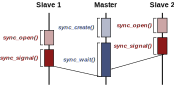
\includegraphics[width=\linewidth]{sync-all-to-one.pdf}}%
				\hfill
				\subcaptionminipage[fig:sync-one-to-all]%
					{.6\linewidth}%
					{The Master notifies N Slaves (\texttt{ONE\_TO\_ALL}).}%
					{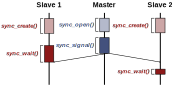
\includegraphics[width=\linewidth]{sync-one-to-all.pdf}}%

				\fonte{Developed by the Author.}%
			\end{figure}

			\subsubsection{Receiver Side Implementation}

% O que é a interface?
% Quais são os parâmetros para realizar uma operação?
				% O Codigo 4 apresenta a interface Sync para nós receptores proposta para o Nanvix HAL. Os parâmetros necessário para a abertura de um ponto de sincronização é uma lista de IDs lógicos, o tamanho da lista e o tipo de sincronização. A lista deve ser sempre inicializada com o ID do nó mestre, independentemente do modo. Os identificadores restantes, contando que não tenham repetição, podem estar em qualquer ordem. O tipos de sincronização são os modos descritos anteriormente definidos através de constantes. As demais funções utilizam o identificador da abstração retornado pela função de criação. Caso algum parâmetro esteja em desacordo ou inválido, um valor negativo é retornado indicando o erro, \eg, \texttt{nodes == NULL}.

				\autoref{code:hal-sync-receiver} introduces the Sync Interface for Receiver Nodes proposed for the \nanvix \hal. The parameters required for creating a sync point are a list of logical IDs, list size, and mode of synchronization. The list must always be initialized with the master node ID, regardless of mode. The remaining identifiers, provided they have no repetition, can be in any order. The other functions use the abstraction identifier returned by the create function. If any parameters are in disagreement or invalid, a negative value is returned indicating the error, \eg nodes pointer equal to \texttt{NULL}.

\begin{listing}[!tb]
\caption{Nanvix HAL: Sync Interface for Receiver Node.}
\label{code:hal-sync-receiver}
\begin{minted}{c}
/**
 * @brief Allocates and configures the receiving side of
 * the synchronization point.
 */
int sync_create(const int *nodes, int nnodes, int mode);

/* @brief Releases and cleans receiver slot. */
int sync_unlink(int syncid);

/* @brief Waits a signal. */
int sync_wait(int syncid);
\end{minted}
\fonte{Developed by the Author.}
\end{listing}

% Quais recursos são necessário para cada tipo de operação, envio e recebimento?
				% O recebimento das notificações requer a reserva 1 slot rx da CNoC relativo ao identificador do mestre. Deste modo, eliminamos o conflito no uso de diferentes slots por diferentes configurações de sincronização. Em contrapartida, um nó não poderá ser o mestre em duas operações simultâneas. O total de abstrações que podem ser criadas desta maneira é igual a quantidade de nós existentes (24 no MPPA). Nos cluster I/O, este total é multiplicado pelo número de interface NoC disponíveis, ou seja, 24 por DMA. A configuração do slot é realizado através de uma máscara de 64-bits. Está mascará é construida com os IDs lógicos dos emissores de modo que os bits relativos a suas posições sejam iguais a 0. Ao receber um sinal, a DMA realiza um OR com o valor anterior. Quando todos os bits se tornarem 1's, a DMA zera todos os bits do registrador e emite uma interrupção.

% Como as operações funcionam?
				% Um vetor de estruturas internas realiza o controle das operações. Cada posição do vetor é reservado a um slot físico e guarda flags de controle, a mascará e um spinlock. Ao realizar a abertura, espera ou unlink de um sync, a HAL verifica discrepâncias nos IDs, nas flags de controle ou nos parâmetros. Por fim, o spinlock é utilizado para sincronização da operação com os núcleos escravos. Em um sistema microkernel, o core mestre configura o sync e o escravo aguarda ser liberado no spinlock. O tratador de interrupções do Sync identifica a estrutura e libera o bloqueio. A falta de coerência de cache não afeta os spinlock porque são utilizadas instruções que garantem a atomicidade que implementam o lock.

				Receipt of notifications requires booking 1 \cnoc RX slot related to the Master ID. This relation eliminates the conflict of using a same slot across different synchronization settings. Consequently, a node cannot be the master in two simultaneous operations. Thus, the total of \sync created simultaneously is equal to the number of existing nodes, \ie 24 in \mppa. In \ioclusters, this total is multiplied by the number of available NoC interfaces, \ie 24 per \dma. A 64-bit mask, created from sender node IDs, configures the RX slot. Bits positioned on nodes IDs are 0. When receiving a signal, \dma performs an \textit{OR-bitwise} with the previous value. When all bits become 1's, \dma clears the register and triggers an interrupt.

				A vector of internal structures controls the operations. Each structure is reserved for a physical slot and holds control flags, the initial mask, and a spinlock. \hal checks for discrepancies in IDs, control flags, or parameters when creating, waiting, or unlinking a \sync. Finally, the spinlock is used to synchronize the operation with slave cores. On a microkernel-based system, the master core configures \sync, and the slave waits for the spinlock release. The interrupt handler of the \sync identifies the structure and releases the lock. The lack of cache coherence does not affect spinlocks because instructions that guarantee the atomicity are used to implement the lock.

% Como foi resolvido o problema de multiplos nós nos IOs? PRECISA FALAR? DARIA PRA ARRUMAR ISSO NO CÓDIGO FORÇANDO QUE O ID[1] FOSSE O ID LOCAL (CASO NAO FOR O MESTRE).
				% A lista de nós foi projetada para utilizar os IDs das interfaces NoCs ao invés dos IDs dos Cluster para não desperdiçar as DMAs extras existentes nos Cluster I/O.

			\subsubsection{Sender Side Implementation}

% O que é a interface?
% Quais são os parâmetros para realizar uma operação?
				% A interface do nó emissor, apresentada pelo Código 3, utiliza os mesmo parâmetros para abertura de um sync. Ao utilizar os mesmo valores na criação e abertura, a aplicação cliente pode definir o papel do cluster simplemente definindo qual função deve ser chamada. Entretanto, tanto na criação quanto na abertura, o ID lógico local deve estar Range correto do lista. Por exemplo, um sync é aberto com o ID local como mestre mas o tipo de sincronização é definido como ALL\_TO\_ONE. Isto retornará um erro e o sync não será aberto porque o mestre deveria ser o receptor das notificações e não o emissor. O restante da implementação segue o que já foi explicado na seção anterior.

				The Sync Interface for Sender Nodes, presented by \autoref{code:hal-sync-sender}, uses the same create parameters for opening a \sync point. The standardization of parameters simplifies the role of a cluster in a synchronization. However, at both creation and opening, the local ID must be included in the list. For instance, a \sync opened with the local ID as master, but the mode defines \texttt{ALL\_TO\_ONE} behavior. This discrepancy will return an error because the master should be the notification receiver and not the sender. The rest of the implementation follows what was already explained in the previous section.

\begin{listing}[!tb]
\caption{Nanvix HAL: Sync Interface for Sender Node.}
\label{code:hal-sync-sender}
\begin{minted}{c}
/**
 * @brief Allocates and configures the sending side of
 * the synchronization point.
 */
int sync_open(const int *nodes, int nnodes, int mode);

/* @brief Releases the transfer channel. */
int sync_close(int syncid);

/* @brief Sends a signal. */
int sync_signal(int syncid);
\end{minted}
\fonte{Developed by the Author.}
\end{listing}

% Quais recursos são necessário para cada tipo de operação, envio e recebimento?
% Como as operações funcionam?
				% De maneira oposta ao receptor, o emissor necessita de 1 canal de envio da CNoC para abrir um sync. Devido a separação dos canais descritos na seção (MPPA HARDWARE), um nó só poderá abrir um sync por vez. Para emitir um sinal, o nó precisa identificar o ID lógico e o slot de recebimento do mestre. A mascará que será ser enviada é sempre um valor de 64-bits com o bit relativo ao nó emissor setado como 1. A estrutura de controle do emissor também possui flags para garantir a semântica das operações. Somado a isso, o emissor guarda, em um array de inteiros, todos os IDs lógicos dos destinatário do sinal. Ao performar de fato o envio, será configurado e enviado um sinal para cada target desta lista. O envio do sinal é realizado através da escrita em um registrador da DMA, desta maneira, não é possível realizar esta ação de forma assíncrona como as demais abstrações.

				Unlike the receiver, the sender needs 1 \cnoc TX channel to open a \sync point. Due to the separation of channels described in the \autoref{tab.noc-resources}, a node can only open one \sync at a time. The node must identify the target ID and RX slot of the master to emit a signal. A 64-bit value composes the mask with the sender node bit set to 1. The sender control structure also has flags to ensure the semantics of the operations. Besides, the sender stores, in an array of integers, all IDs of the receivers. When performing the notification, a signal will be sent to each target of this list.

		\subsection{Mailbox Abstraction}
		\label{sec.mailbox-abs}


			% The \textit{Mailbox Abstraction} allows clusters to exchange fixed-size
			% messages with each other.
			% The message was thought to be a relatively small size, usually a few hundred bytes.
			% Similarly, the operation of the \mailbox follows \posix message queue behavior.
			% For example, the message can be used to encode small operations and system
			% control signals.
			% As illustrated in \autoref{fig:mailbox}, the operation cardinality is N:1,
			% where N senders can transfer one message at a time to a receiver queue.
			% When the receiver consumes a message, it notifies the sender to ensure
			% control of the flow.

			% A abstração \textit{Mailbox} permite que clusters troquem mensagens de tamanho fixo entre si. O tamanho da mensagem foi projetado para ser relativamente pequeno, geralmente algumas centenas de bytes. Essas mensagens são consumidas pelo receptor sem a necessidade de conhecer quem as enviou. Similarmente, a operação da \mailbox segue o comportamento da fila de mensagens \posix. A Figura (conceito) ilustra conceitualmente uma das formas de implementar uma Mailbox. O receptor aloca espaço suficiente para receber 1 mensagem de cada possível emissor. O emissor envia para o espaço reservado para sua mensagem, eliminando a concorrência de escrita das mensagens.

			Mailbox abstraction allows clusters to exchange fixed-length messages with each other. The message size is designed to be relatively small, usually a few hundred bytes. The recipient consumes these messages without needing to know who sent them. Similarly, the mailbox operation follows the behavior of the Posix message queue. Figure (concept) conceptually illustrates one of the ways to implement a Mailbox. The receiver allocates enough space to receive one message from each possible sender. The sender transfers the message to a predefined location.

			\begin{figure}[!tb]
				\centering%
				\caption{Mailbox Abstraction Concept.}%
				\label{fig:mailbox}%

				\subcaptionminipage[fig:mailbox-concept]%
					{.4\linewidth}%
					{Conceptual Overview.}%
					{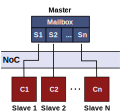
\includegraphics[width=\linewidth]{mailbox-concept.pdf}}%

				\hfill

				\subcaptionminipage[fig:mailbox-flow]%
					{.5\linewidth}%
					{Flow of execution: Slave sends a message, Master reads and notifies the sender.}%
					{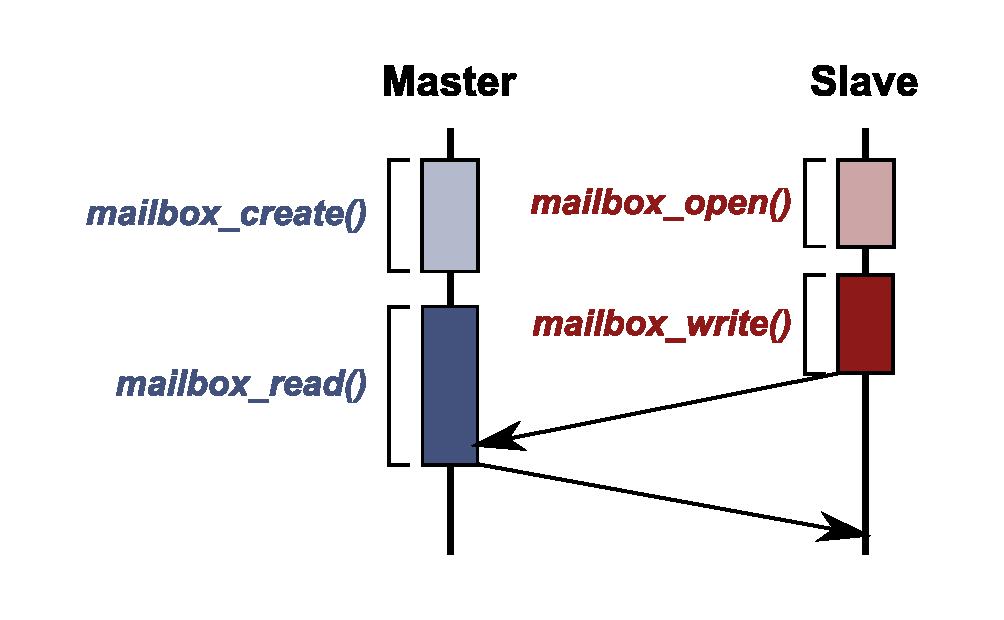
\includegraphics[width=\linewidth]{mailbox-flow.pdf}}%

				\fonte{Developed by the Author.}%
			\end{figure}

			% A Figura (fluxo) exemplifica o fluxo de comunicação entre um nó receptor e um emissor. A criação de uma Mailbox cria uma fila de mensagens vazia, onde os emissores são livres para enviar a primeira mensagem. Posteriormente, todos os envios necessitaram da permissão do receptor para que mensagens não sejam sobreescritas. Por este motivo, o receptor notificará o emissor ao consumir sua mensagem. A mensagem será copiada para um buffer do usuário e o espaço estará novamente disponível.

			% Teoricamente, a quantidade de mensagens permitidas por emissor pode ser de 1 à N. Entretanto, optou-se por permitir apenas 1 no Nanvix HAL devido as restrições de memória apresentada por manycores. E como o espaço é alocado estatícamente dentro do espaço de memória do kernel, permitir que o usuário escolhe-se o tamanho da fila de mensagem não reduziria o espaço prévio necessário. Todavia, o uso de uma mensagem é suficiente para programas servidores tratarem requisitações no nível do Multikernel. Por exemplo, a mensagem pode ser usada para codificar pequenas operações e sinais de controle do sistema.

			Figure (flow) exemplifies the communication flow between a receiver and a sender node. The receiver creates an empty message queue where senders are free to send the first message. Subsequently, in order not to overwrite old messages, all transmissions require the permission of the receiver. For this reason,  when the receiver consumes a message, it copies the message to the user buffer, releases the queue space, and notifies the sender.
			
			Theoretically, the number of messages allowed per sender can be from 1 to N.  However, Nanvix HAL statically allocates sufficient memory for the message queue inside the kernel. Therefore, we chose to allow only one message due to memory constraints presented by lightweight manycores. Furthermore, using one message is sufficient for servers to handle requests at the Multikernel level. For instance, the message can be used to encode small operations and system control signals.
			
			\subsubsection{Receiver Side Implementation}

% Interface e seus parâmetros
				O código 3 apresenta a interface da Mailbox para um nó receptor.
				A criação de uma Mailbox requer que a aplicação informe o ID Lógico no nó local.
				Esta identificação é necessária por causa do múltiplos nós existentes nos Cluster I/O.
				As demais operações utilizam o identicador retornado na criação da mailbox.
				Para a leitura de uma mensagem, o usuário é obrigado a passar o local onde a mensagem será copiada e o tamanho a ser copiado.
				O tamanho é sempre constante mas é utilizado como verificação da integridade da operação.
				A cópia bem sucedida de uma mensagem liberará o escravo que executar a função de espera.
				Neste processo de liberação, o core mestre executa o flush da mensagem para a SRAM para que o escravo, ao invalidar a sua cache, possa ler a mensagem.

% Recursos de hardware
				A Mailbox é mais complexa do que o Sync porque utiliza recursos DNoC e CNoC.
				Especificamente, o receptor necessita de 1 slot de recebimento da DNoC e 1 canal de transmissão da CNoC.
				A necessidade de 1 canal de transmissão durante toda a vida da Mailbox do receptor limita a criação de apenas 1 mailbox por nó NoC.
				O slot rx é configurado utilizando dois tamanhos.
				Um para o tamanho de uma mensagem, o qual gerará interrupções, e outro para o tamanho total buffer alocado para proteção.
				O buffer é alocado dentro da memória do kernel com espaço suficiente para receber 24 mensagens.
				A mensagem, propriamente dita, é composta por um cabeçalho identificando o emissor, um corpo contendo a mensagem útil e um rodapé com o mesmo identificador.
				O canal de transmissão, por sua vez, é utilizado após a cópia da mensagem útil para o buffer do usuário, notificando o ID do cabeçalho.

% Desafios da implementação
				O paralelismo no recebimento das mensagens introduziu alguns desafios na leitura assíncrona do Mailbox como 
				(i) cada mensagem gera uma interrupção,
				(ii) interrupções preemptadas por outras não encontraram os recursos da DNoC que emitiram a interrupção e
				(iii) não é possível verificar a quantidade de interrupções geradas por um recurso.
				Para burlar estas barreiras, foi implementado um comportamento similar ao envio preguiçoso.
				Primeiro, um contador global contendo a quantidade total de mensagens recebidas permite que o receptor copie mensagens recebidas antes de uma leitura.
				Segundo, caso não haja mensagens disponíveis, a cópia será realizada pelo próximo disparo do manipulador.
				Terceiro, para resolver o problema das interrupções preemptadas, sempre que um manipulador é disparado ele percorrerá a fila de mensagens conferindo os cabeçalhos e rodapés.
				Ao identificar uma mensagem válida, o manipulador incrementa o contador e altera o rodapé para um código especifico.
				Desta forma, não perdemos nenhuma mensagem por não tratar uma interrupção.

\begin{listing}[!tb]
\caption{Nanvix HAL: Mailbox Interface for Receiver Node.}
\label{code:hal-mailbox-receiver}
\begin{minted}{c}
/* @brief Creates a mailbox. */
int mailbox_create(int nodenum);

/* @brief Destroys a mailbox. */
int mailbox_unlink(int mbxid);

/* @brief Reads data asynchronously from a mailbox. */
ssize_t mailbox_aread(int mbxid, void * buffer, size_t size);

/* @brief Waits for an asynchronous operation to complete. */
int mailbox_wait(int mbxid);
\end{minted}
\fonte{Developed by the Author.}
\end{listing}

			\subsubsection{Sender Side Implementation}

% Interface e seus parâmetros
				O código 3 apresenta a interface da mailbox para o nó emissor.
				A abertura de uma mailbox requer que a aplicação informe o ID lógico do nó que irá receber a mensagem.
				O identificador da mailbox retornado pela função de abertura é utilizada para configurar e controlar as demais funções.
				A função de envio, em especial, implementa o conceito de envio preguiçoso.
				Ou seja, o core mestre nunca ficará bloqueado caso a mailbox não tenha permissão para enviar a mensagem.
				Ele realiza o agendamento do envio setando valores nas estruturas internas do kernel e copiando a mensagem útil para um buffer local, no qual consta o identificador do emissor.
				A função de espera é a mesma função utilizada pelo nó receptor onde o núcleo escravo aguardaram bloqueado em um spinlock até receber a permissão de envio.

				% If the sender attempts to send a message before the receiver has consumed
				% the previous message, the sender will be blocked waiting for the sender's notification.
				% In this way, flow control is guaranteed, and the sender will not overwrite
				% messages unread by the receiver.

\begin{listing}[!tb]
\caption{Nanvix HAL: Mailbox Interface for Sender Node.}
\label{code:hal-mailbox-sender}
\begin{minted}{c}
/* @brief Opens a mailbox. */
int mailbox_open(int nodenum);

/* @brief Closes a mailbox. */
int mailbox_close(int mbxid);

/* @brief Writes data asynchronously to a mailbox. */
ssize_t mailbox_awrite(int mbxid, const void * buffer, size_t size);

/* @brief Waits for an asynchronous operation to complete. */
int mailbox_wait(int mbxid);
\end{minted}
\fonte{Developed by the Author.}
\end{listing}

% Recursos de hardware
				O lado emissor também exige a alocação de recursos das duas NoCs.
				Porém, os recursos são opostos ao do receptor, no qual serão alocados 1 slot rx da CNoC e 1 canal de transmissão da DNoC.
				O slot rx CNOC alocado é relativo ao ID do receptor para evitar que aberturas para receptores distintos conflitassem ao tentar alocar o mesmo slot.
				O canal de transmissão é alocado dinamicamente dentre os 4 disponíveis.
				Deste modo, a quantidade máximo de mailboxes abertas por nó é limitado pelo número de canais de transmissão.

		\subsection{Portal Abstraction}
		\label{sec.portal-abs}

			% \begin{figure}[!tb]
			% 	\centering%
			% 	\caption{Portal Abstraction Concept: Node 1 create a portal and notify Node 2 to transfer the data.}%
			% 	\label{fig:portal}%
			% 	\includegraphics[width=.65\textwidth]{.pdf}%
			% 	\fonte{Developed by the Author.}%
			% \end{figure}

% Apresentação do portal e o conceito.
			Por fim, a abstração Portal permite que dois nós troquem quantidades arbitrárias de dados.
			A Figura (conceito) apresenta a ideia conceitual do portal, onde se assemelha a do POSIX Pipes com controle de fluxo.
			A cardinalidade das operações é sempre 1:1, onde um par de nós abre um canal unidirecional para transferência de dados.
			Porém, ao contrário do POSIX Pipes que define que o pipe existe apenas entre dois processos, o portal permite que o receptor se comunique com outros nós através de um mesmo canal.
			O emissor, por sua vez, poderá apenas se comunicar com um nó.

% Fluxo da operação
			A Figura (fluxo) exemplifica o controle de fluxo proposto para o portal.
			Ao tentar transmitir dados ao receptor, o emissor blorqueará até que o receptor esteja apto à receber.
			O receptor, ao habilitar uma troca de dados de cada vez, configura a leitura e notifica o emissor.
			Deste modo, o controle de fluxo garante que o receptor não será sobrecarregado, não receberá dados sem que a DMA esteja devidamente configurada, e não sobrescreverá dados prévios.
			O ato de habilitar uma comunicação permite que o receptor escolha com qual nó deseja se comunicar.

% Diferença do posix, receptor allows multiples issuers

			\begin{figure}[!tb]
				\centering%
				\caption{Portal Abstraction Concept.}%
				\label{fig:portal}%

				\subcaptionminipage[fig:portal-concept]%
					{.4\linewidth}%
					{Conceptual Overview.}%
					{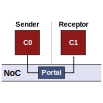
\includegraphics[width=\linewidth]{portal-concept.pdf}}%

				\hfill

				\subcaptionminipage[fig:portal-flow]%
					{.5\linewidth}%
					{Node 1 create a portal and notify Node 2 to transfer the data.}%
					{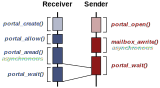
\includegraphics[width=\linewidth]{portal-flow.pdf}}%

				\fonte{Developed by the Author.}%
			\end{figure}

			\subsubsection{Receiver Side Implementation}

% Interface e seus parâmetros
				O Código 5 apresenta a interface portal para nós receptores.
				Assim como a mailbox, a aplicação deve identificar o nó local para criar um portal.
				As demais funções utilizam o identificador do portal retornado pela função de criação.
				Para criar um canal de comunicação, o receptor sempre deverá executar 3 operações, allow, aread, wait.
				A função allow aloca um slot rx relativo ao nó remoto informado, limitando um canal por par de nós.
				Entretanto, a notificação apenas será enviada, relativo ao nó remote, após a configuração da DMA pela função aread.
				Por fim, o nó bloqueará na função wait até a comunicação ser completada.

% Recursos de hardware
				Um portal receptor aloca um slot rx da DNoC e um canal tx da CNoC.
				Diferente da mailbox, o portal tem disponível 2 canais tx o que permite a criação de dois portais simultâneos.
				Tais portais não podem se comunicar com o mesmo nó ao mesmo tempo por causa da escolha do slot físico da DMA comentado no parágrafo anterior.
				A leitura configura o slot rx com o buffer e tamanho informado pela aplicação.
				Isto elimina as cópias intermediárias como da mailbox, onde a DMA escreve os dados direto no buffer da aplicação.
				As estruturas de controle também são simplificadas por causa disso
				contendo apenas flags e um spinlock liberado pelo manipulador do portal.

\begin{listing}[!tb]
\caption{Nanvix HAL: Portal Interface for Receiver Node.}
\label{code:hal-portal-receiver}
\begin{minted}{c}
/* @brief Creates a portal. */
int portal_create(int local);

/* @brief Destroys a portal. */
int portal_unlink(int portalid);

/* @brief Allow sender to transfer data. */
int portal_allow(int portalid, int remote);

/* @brief Reads data asynchronously from a portal. */
ssize_t portal_aread(int portalid, void * buffer, size_t size);

/* @brief Waits for an asynchronous operation to complete. */
int portal_wait(int portalid);
\end{minted}
\fonte{Developed by the Author.}
\end{listing}

			\subsubsection{Sender Side Implementation}

% Interface e seus parâmetros
				O código 6 apresenta a interface portal para nós emissores.
				Na abertura de um portal, a aplicação é obrigada a informar o nó local e o nó remote que receberá os dados.
				O id local serve para distinguir a interface NoC casa haja multiplos nó em um cluster e o id do nó remote será utilizado para alocar e configurar o slot rx da CNoC que receberá a permissão de transferência.
				Isto garante que a permissão não será perdida, mesmo se a permissão chegar antes do emissor configurar a escrita.
				Os dados são transferidos seguindo o algoritmo de envio preguiçoso.

% Recursos de hardware
				Os recursos de hardware necessários para abrir um portal são opostos ao recursos de criação.
				Especificamente, são necessários 1 slot rx da CNoC e 1 canal tx da DNoC.
				O slot rx está apto a receber a permissão desde a abertura do portal.
				O canal de transmissão é reservado mas só é utilizado quando for permitido o envio.
				Devido a limitação de 4 canais tx para o portal, apenas 4 portais emissores podem ser abertos ao mesmo tempo.
				A estruturas de controle para os portais emissores contém os parâmetros necessário para realizar o envio preguiçoso e um spinlock para controlar o término da operação de transferência.

\begin{listing}[!tb]
\caption{Nanvix HAL: Portal Interface for Sender Node.}
\label{code:hal-portal-sender}
\begin{minted}{c}
/* @brief Opens a portal. */
int portal_open(int local, int remote);

/* @brief Closes a portal. */
int portal_close(int portalid);

/* @brief Writes data asynchronously to a portal. */
int portal_awrite(int portalid, const void * buffer, size_t size);

/* @brief Waits for an asynchronous operation to complete. */
int portal_wait(int portalid);
\end{minted}
\fonte{Developed by the Author.}
\end{listing}

				\todo[inline]{Trabalhos futuros: Eliminar a necessidade de informar o remote na abertura criando um função allow igual o reciever.}

	\section{User-Level Communication}
	\label{sec.comm-services}
	\todo{Or: Nanvix Microkernel Level}

		The inter-cluster communication module, described in \autoref{sec.low-level-comm},
		is designed to export a standard and straightforward communication
		primitives to different lightweight manycores.
		These primitives can be used by various types of \oss and applications.
		Thus, the module is flexible enough not to impact the performance
		of the upper layers negatively.
		For this, it does not provide rich management of the exposed abstractions.

		In this scenario, the communication services of \nanvix \microkernel seek
		to provide \ipc between distinct clusters.
		Specifically, these services perform the multiplexing of the hardware
		resources and the verification of the parameters that will be passed
		on the communication primitives.
		Due to the Master-Slave model, the responsibility of protecting,
		manipulating, and configuring \hal resources is of the master core.
		The slave core will request operations through the system call interface,
		passing the necessary information to the master.

		Considering that the abstractions make up the fundamental elements of
		the construction of more complex services, the \microkernel services
		were responsible for the management and multiplexing of the finite
		resources for the many cores of a cluster.
		In total, there are three communication services in the \nanvix \microkernel,
		each associated with an abstraction of the communication module,
		analogously named \sync, \mailbox, and \portal services.
		These services must take into account the memory constraints and the
		Master-Slave model chosen for the \microkernel.

		The impacts of the Master-Slave model, protection, management and manipulation 
		operations are similar to all services.
		Thereat, the following sections provide an overview of these topics punctuating 
		the differences of each service.

		They will be provided through interfaces that function as wrappers
		for the \hal abstraction functions.
		In the implementation of these interfaces, there will be a mapping
		between low-level identifiers, associated with \hal resources,
		and high-level identifiers, associated with resource protection structures.

			% The protection operations are mostly similar.
			% For instance, the use of unallocated resources, sanitizing entries,
			% checking valid identifiers, non-null pointers, and checking
			% for conflicting operations (reading in write-only resources).
			% In the meantime, there are exceptional cases in some services
			% that must be taken.
			% For instance, in the \sync service, a cluster cannot synchronize
			% with itself, or there is a repetition of identifiers in the
			% stipulated set of clusters.

			% Finally, some aspects of services and implementation still need
			% to be analyzed and will be better detailed in another version
			% of the dissertation.
			% For example, what resource multiplexing methods will be used
			% and their impacts on the Nanvix Microkernel services.

		\subsection{Impacts of the Master-Slave Model}

			O modelo mestre-escravo define que as estruturas internas do SO devem ser exclusivamente manipuladas pelo núcleo mestre.
			Para isso, cada serviço possui estruturas genéricas e simples que guardam flags de controle, parâmetros para identificação da recurso e armazenamento dos descritores físicos retornados pela HAL.
			Desta forma, existem dois conjuntos de funções que separa a responsabilidade dos escravos das responsabilidades do mestre.
			A única excessão é a chamada da função de esperar onde ela é inteiramente realizadas pelo núcleo escravo.
			Inclusive, foi possível exportar funções síncronas do lado do escravo ao forçar a espera da conclusão de operações assíncronas em uma chamada de sistema.

			O conjunto de funções do mestre segue a notação \texttt{kernel\_\textbf{abstraction}\_\textit{operation}} e é utilizada pelo mecanismo de chamadas de sistemas para realizar a proteção, manuseio e multiplexação dos serviços.
			O conjunto de funções destinada aos escravos é a interface exportada pelas chamadas de sistemas, definidas como \texttt{k\textbf{abstraction}\_\textit{operation}}.
			Suas responsabilidades é pesquisar qual identificado anexo ao nó local, caso exista mais de um, e realizar os testes de sanidade possíveis do lado do escravo.

			O fato de que o mestre não pode bloquear a espera de uma única operação forçou que a operação da chamada de espera seja realizada pelo escravo.
			Neste ponto, o escravo precisa acessar a estrutura interna do SO para consultar o descritor de baixo nível da abstração para que tenha acesso ao spinlock da HAL.
			Para garantir a coerência da estrutura, o mestre atualiza a memória local sempre que uma modificação é realizada e o escravo invalida sua cache.

		\subsection{Protection and Management}

			As operações de proteção e gerência envolvem duas fases, a fase do escravo e a fase do mestre.
			Na fase do escravo é verificado todos os problemas que poderiam ser detectados antes de requisitar a operação ao mestre.
			Por exemplo,
			(i) descritores de arquivos válidos,
			(ii) ponteiros de buffer não nulos,
			(iii) tamanhos de buffers dentro do limite estipulado, e
			(iv) a semântica dos serviços como sincronização consigo mesmo.
			
			O mestre, além de realizar as mesmas verificações do escravo, tem a responsabilidade de conferir a semântica das operações sobre um determinado recurso.
			Especificamente, o mestre
			(i) identifica multiplas criações/aberturas
			(ii) verifica operações conflitantes, como escritas em recursos configurados apenas para leitura,
			(iii) mensura tempo de comunicação e quantidade total de bytes transmitidos/recebidos, e
			(iv) chama as abstrações da HAL identificando erros retornados.

		\subsection{Multiplexing}

			A identificação de recursos criados/abertos com os mesmo argumentos permite que multiplos escravos utilizem um mesmo recurso em momentos distintos.
			Para isso, as estruturas internas do SO guardam, da forma mais simplificada possível, os argumentos utilizados na criação/abertura de um serviço.
			Quando identificado os mesmos argumentos, um contador de referências é incrementado.
			O mestre configura o recurso como ocupado quando solicitado uma leitura/escrita.
			Um segundo escravo que deseja ler/escrever será impedido até que a operação anterior seja concluida.
			A liberação dos recursos da HAL só seram liberados quando todas as referências forem removidas.

		\subsection{Input/Output Control}

			Os serviços de mailbox e portal contam com uma chamada de sistema especial, chamada de \ioctl.
			Essas chamada concede a implementação de operações que não podem ser expressadas por chamadas de sistemas regulares.
			No caso dos serviços de comunicação, 2 tipos de operações foram implementadas.
			A primeira operação, denominada \texttt{IOCTL\_GET\_VOLUME} consulta a quantidade atual de bytes transmitidos/recebidos de um serviço.
			A segunda operação, denominada \texttt{IOCTL\_GET\_LATENCY}, consulta a soma das latências das comunicações mensuradas através da diferença de duas leituras de clock.
			Essa chamada de sistema pode ser extendida futuramente para introduzir novas funcionalidades e operações sem causar mudanças nas interfaces atuais.

		\subsection{Validation and Correctness Tests}

			A validação e teste de corretude da implementação dos serviços foi realizada através de 2 conjunto de testes unitários, testes de API e testes de FALHA, respectivamente.
			Por um lado, os testes de API criam, abrem e estimulam os serviços com argumentos dentro dos intervalos de valores válidos.
			Por outro lado, os testes de FALHA utilizam argumentos fora do intervalo de domínio das operações.
			A falha deve gerar um valor de erro previamente conhecido.
			Os testes validam qualquer mudança feita verificando todos os comportamentos esperados pelos serviços.
